\documentclass[border=5pt]{standalone}
\usepackage{amsmath}
\usepackage{tikz}
\usetikzlibrary{positioning, fit, shapes, arrows}
\usetikzlibrary{chains}
\usetikzlibrary{calc}
\usetikzlibrary{decorations.pathmorphing}
\usetikzlibrary{decorations.pathreplacing}
\usetikzlibrary{shapes.multipart}
\begin{document}

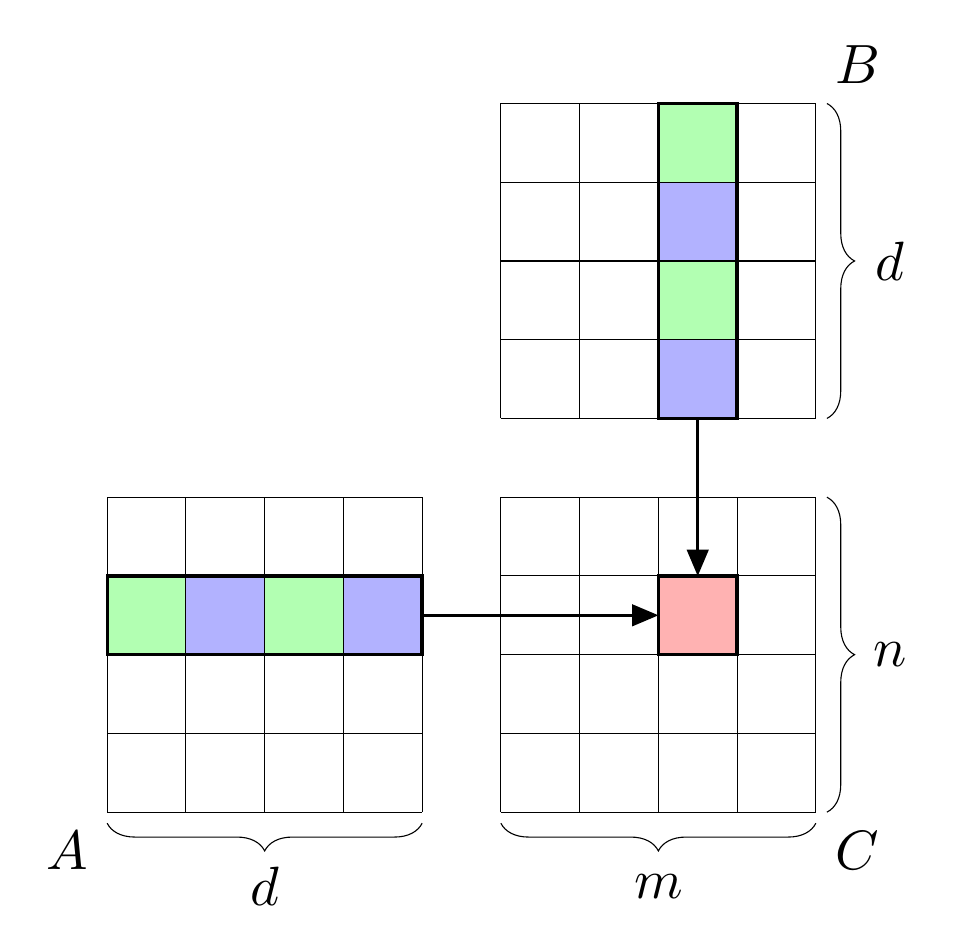
\begin{tikzpicture}[node distance=0.15 cm, font=\sffamily]

% Bunte Felder
%\fill[color=gray!20] (4,0) rectangle (8,4);

% A
\begin{scope}[xshift=-5cm]
  \fill[color=green!30] (0,2) rectangle (1,3);
  \fill[color=blue!30] (1,2) rectangle (2,3);
  \fill[color=green!30] (2,2) rectangle (3,3);
  \fill[color=blue!30] (3,2) rectangle (4,3);

  \draw[step=1cm,black,thin] (0,0) grid (4,4);
  
	\draw[very thick] (0,2) rectangle (4,3); % row

  \node[anchor=north east, scale=2] at (0,0) {$A$};

  %\node[draw, circle, minimum size=20pt, line width=1.2, fill=green!30]
  %      (m) at (0.5,2.5) {};
  %\node[scale=1.75] at (m.center) {1};
  %\node[draw, circle, minimum size=20pt, line width=1.2, fill=blue!30]
  %      (m) at (1.5,2.5) {};
  %\node[scale=1.75] at (m.center) {2};
  %\node[draw, circle, minimum size=20pt, line width=1.2, fill=green!30]
  %      (m) at (2.5,2.5) {};
  %\node[scale=1.75] at (m.center) {3};
  %\node[draw, circle, minimum size=20pt, line width=1.2, fill=blue!30]
  %      (m) at (3.5,2.5) {};
  %\node[scale=1.75] at (m.center) {4};

  \draw [decorate,decoration={brace,mirror,amplitude=10pt},yshift=-4pt,xshift=0pt]
    (0,0) -- (4,0) node [black,midway,yshift=-0.8cm,scale=2]  {$d$};
\end{scope}

% B
\begin{scope}[yshift=5cm]
  \fill[color=green!30] (2,3) rectangle (3,4);
  \fill[color=blue!30] (2,2) rectangle (3,3);
  \fill[color=green!30] (2,1) rectangle (3,2);
  \fill[color=blue!30] (2,0) rectangle (3,1);

  \draw[step=1cm,black,thin] (0,0)grid(4,4);

	\draw[very thick] (2,0) rectangle (3,4); % column

  \node[anchor=south west, scale=2] at (4,4) {$B$};

  %\node[draw, circle, minimum size=20pt, line width=1.2, fill=green!30]
  %      (n) at (0.5,3.5) {};
  %\node[scale=1.75] at (n.center) {1};
  %\node[draw, circle, minimum size=20pt, line width=1.2, fill=blue!30]
  %      (n) at (0.5,2.5) {};
  %\node[scale=1.75] at (n.center) {2};
  %\node[draw, circle, minimum size=20pt, line width=1.2, fill=green!30]
  %      (n) at (0.5,1.5) {};
  %\node[scale=1.75] at (n.center) {3};
  %\node[draw, circle, minimum size=20pt, line width=1.2, fill=blue!30]
  %      (n) at (0.5,0.5) {};
  %\node[scale=1.75] at (n.center) {4};

  \draw [decorate,decoration={brace,mirror,amplitude=10pt},xshift=4pt,yshift=0pt]
    (4,0) -- (4,4) node [black,midway,xshift=0.8cm,scale=2]  {$d$};
\end{scope}

% C
\begin{scope}[]
  \fill[color=red!30] (2,2) rectangle (3,3);

  \draw[step=1cm,black,thin] (0,0) grid (4,4);

	\draw[very thick] (2,2) rectangle (3,3); % red element

  \node[anchor=north west, scale=2] at (4,0) {$C$};

  %\node[draw, circle, minimum size=20pt, line width=1.2, fill=red!30]
  %      (d) at (0.5,3.5) {};
  %\node[scale=1.75] at (d.center) {R};

  \draw [decorate,decoration={brace,mirror,amplitude=10pt},xshift=4pt,yshift=0pt]
    (4,0) -- (4,4) node [black,midway,xshift=0.8cm,scale=2]  {$n$};

  \draw [decorate,decoration={brace,mirror,amplitude=10pt},yshift=-4pt,xshift=0pt]
    (0,0) -- (4,0) node [black,midway,yshift=-0.8cm,scale=2]  {$m$};

  \begin{scope}[very thick]	
	  \draw[->, >=triangle 45] (-1,2.5) -- (2,2.5);
  	\draw[->, >=triangle 45] (2.5,5) -- (2.5,3);
  \end{scope}
\end{scope}

% arrows





    
\end{tikzpicture}
\end{document}
